\documentclass{beamer}

\usetheme[sectionpage=progressbar,subsectionpage=progressbar,numbering=fraction,
          progressbar=foot]{metropolis}

\graphicspath{{../img/}}

\usepackage{appendixnumberbeamer}

\usepackage{datetime}
\newdate{defensedate}{31}{01}{2018}
\newdate{startdate}{07}{02}{2018}
\newdate{enddate}{22}{06}{2018}

\usepackage{minted}
\usepackage{inconsolata}
\setmonofont{Inconsolatazi4}

\usepackage{textcomp}

\usepackage{xpatch}
\usepackage[citestyle=authortitle,backend=bibtex]{biblatex}
\addbibresource{../bibl.bib}
\xapptobibmacro{cite}{\setunit{\nametitledelim}\printfield{year}}{}{}
% \usepackage{chngcntr}
% \counterwithin*{footnote}{page}

\title{Search-Based Test Amplification\\\large{COLQ --- M2 SIF}}
\subtitle{Supervisor: Benoit Baudry\\KTH, Sweden\\\displaydate{startdate} -- \displaydate{enddate}}

\date{\displaydate{defensedate}}
\author{%
  Simon Bihel\hfill\url{simon.bihel@ens-rennes.fr} \\
}
\institute{%
  University of Rennes I \\
  \'Ecole Normale Sup\'erieure de Rennes
}

\begin{document}

\maketitle

\section{Introduction}

\begin{frame}{Test Suites}
  Context:
  \begin{itemize}
    \item Software projects are now accompanied by strong test suites
    \item Takes time to write
    \item Still missing some bugs due to focus on nominal paths when writing test cases
  \end{itemize}

  \pause{}

  Related works:
  \begin{itemize}
    \item Measure the quality of test suites
    \item Automatically write test suites
    \item \alert{Amplify} existing test suites
  \end{itemize}
\end{frame}

\begin{frame}{Concepts}
  System-Under-Test: function, class, whole program...
  \begin{description}
    \item[Inputs] E.g.\ function parameters, method calls to setup and stimulate an object
    \item[Assertions] Used to test whether the function's output is correct, that the object is in the right state
  \end{description}
\end{frame}
\begin{frame}[fragile]{Test Example}
  \begin{minted}[linenos]{java}
testIterationOrder() {
  TreeList tl = new TreeList(10);
  for (int i = 0; i < size; i++) {
    tl.add(i);
  }
  int i = 0;
  ListIterator it = tl.listIterator();
  while (it.hasNext()) {
    Integer val = it.next();
    assertEquals(i++, val.intValue());
  }
}
  \end{minted}
\end{frame}

\begin{frame}{Metrics for Test Suites}
  \metroset{block=fill}
  \begin{block}{Goal}
    Detect parts that are not tested.
  \end{block}

  \pause{}

  \begin{exampleblock}{Code Coverage}
    Number of instructions or branches executed by the test suite.
  \end{exampleblock}

  \pause{}

  \begin{exampleblock}{Mutation Score}
    \begin{enumerate}
      \item Create \emph{mutants} (i.e.\ bugged versions) of the main software (e.g.\ change a \texttt{>} with a \texttt{<=}).
      \item Count how many mutants for which the test suite fail.
    \end{enumerate}
  \end{exampleblock}
\end{frame}

\begin{frame}{Automated Test Generation}
  \metroset{block=fill}
  \begin{block}{Goal}
    Generate tests from scratch to fulfill a given metric.

    Large search space of instructions and values.
  \end{block}

  \begin{exampleblock}{Search-based techniques~\footcite{mcminn2011search,fraser2011evosuite}}
    Random, iterative and heuristic-based techniques (e.g.\ Genetic Algorithms, simulated annealing).
  \end{exampleblock}

  \pause{}

  \begin{block}{The oracle problem~\footcite{barr2015oracle}}
    What should the output of a test be?

    \begin{itemize}
      \item Avoid this by focusing on regression testing.
    \end{itemize}
  \end{block}
\end{frame}


\section{Test Suite Amplification}

\begin{frame}{Motivations~\footcite{danglot2017emerging}}
  \begin{itemize}
    \item Reduce search-space by using the existing test suite as a (good) starting population.
    \item Use knowledge in hand-written tests for a better oracle.
  \end{itemize}
\end{frame}

\begin{frame}{Test Data Regeneration~\footcite{yoo2012test}}
  \metroset{block=fill}
  \begin{block}{Goal}
    Modify a test case while keeping the same branch coverage.
    \begin{itemize}
      \item Avoids over-fitting.
      \item Helps for fault detection.
    \end{itemize}
  \end{block}

  \vfill

  Test cases are vectors of integers.
  Modified tests are called \emph{neighbors}.
\end{frame}

\begin{frame}{Test Data Regeneration}
  Modification \emph{operator}:
  \begin{itemize}
    \item $+ 1$ and $- 1$
    \item $* 2$ and $\lceil / 2\rceil$
  \end{itemize}

  \pause{}

  Reduces the search space with a \emph{Search Radius}:
  \begin{itemize}
    \item Move further away from original test.
    \item Limit the number of modifications to avoid searching too far.
  \end{itemize}

  \vfill

  Experiments needed to find best values.
\end{frame}

\begin{frame}{DSpot~\footcite{baudry2015dspot}}
  \metroset{block=fill}
  \begin{block}{Goal}
    Create tests for undetected mutants.
  \end{block}
  \begin{center}
    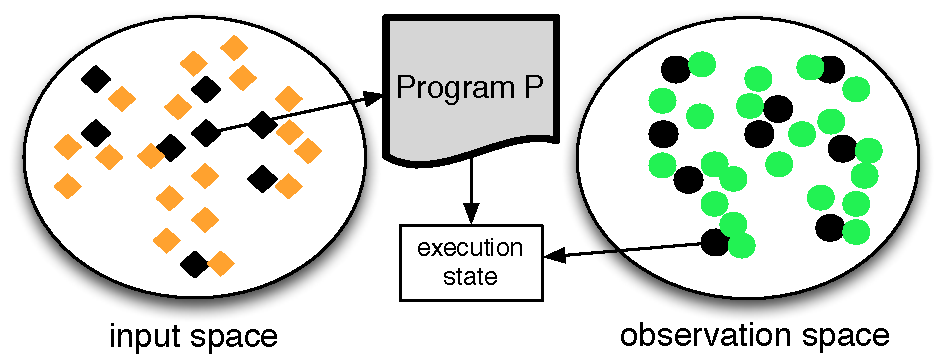
\includegraphics[scale=0.45]{io-spaces.pdf}

    % \fbox{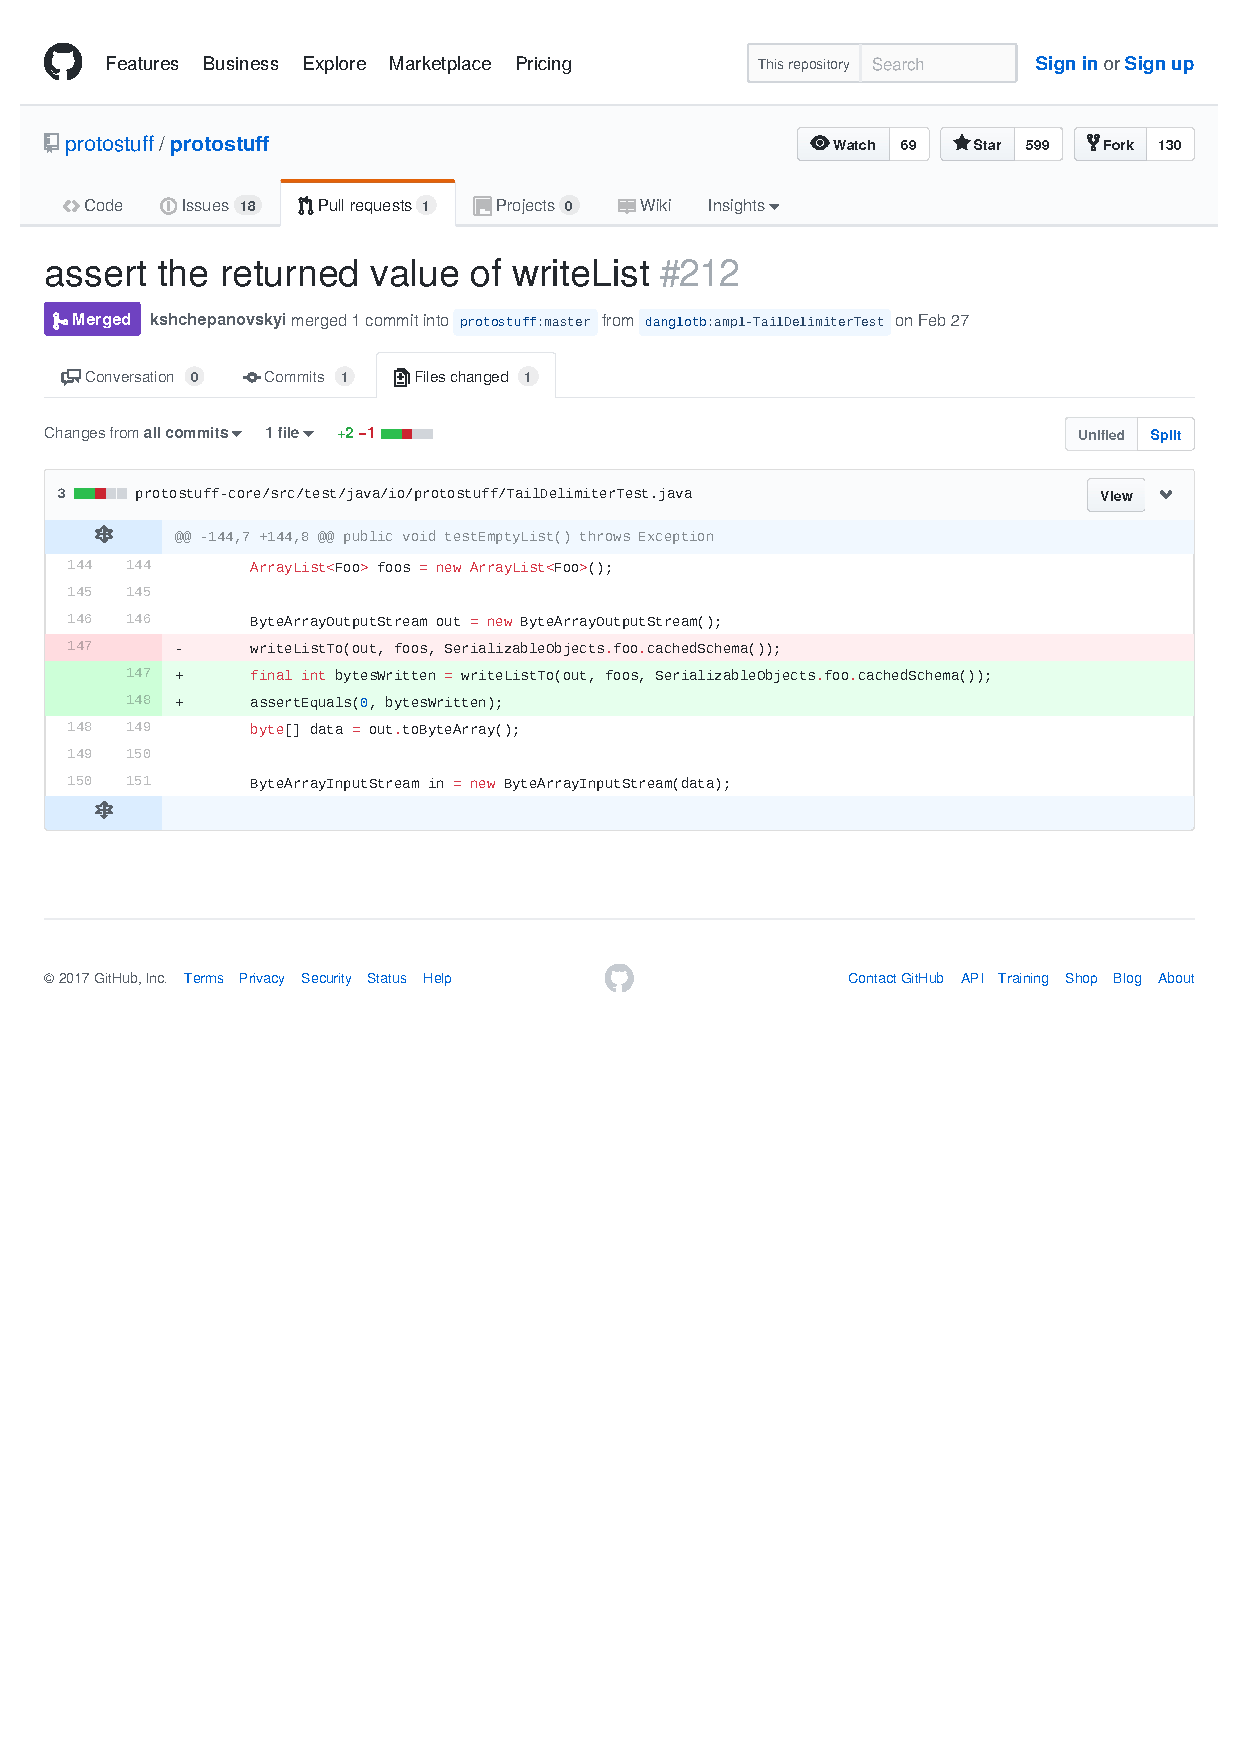
\includegraphics[trim=2cm 17.02cm 4.09cm 10.46cm, clip, width=\textwidth]{rq3_resources/protostuff.pdf}}
  \end{center}
  \pause{}
  \alert{New tests ought to be approved by the developers.}
  Do not mess with people's code.
\end{frame}

\begin{frame}{DSpot --- Amplification Operators}
  \metroset{block=fill}
  \begin{block}{Input amplification}
    \textbf{Literals \textrightarrow{}} replaced with neighbor values.

    \textbf{Method calls \textrightarrow{}} duplicated, removed or made-up (with random or default parameters).

    \pause{}
    \small{Only one operator can be applied}
  \end{block}

  \vfill
  \pause{}

  \begin{block}{Assertion amplification}
    Capture the state of the system after the test's execution.
  \end{block}
\end{frame}


\section{Planned Work}

\begin{frame}{Easing the Review Process}
  \begin{block}{Human review process}
    \begin{itemize}
      \item Takes time.
      \item Misunderstood tests are ignored or labelled as false-positive.
    \end{itemize}
  \end{block}

  \begin{block}{What we could do}
    \begin{itemize}
      \item Add explanations \textbf{\textrightarrow} easier to understand what the target of the new test is.
      \item Avoid testing completely different things.
      \item Order tests by importance.
    \end{itemize}
  \end{block}
\end{frame}
% modify existing test case or add a new one

\begin{frame}{Efficient Generation}
  Minimal set of tests \textbf{if} each test stays simple and logical.

  \vfill

  \begin{block}{Stacking operators}
    \begin{itemize}
      \item More properties covered.
      \item Increases the search space, study the usefulness of each operator.
    \end{itemize}
  \end{block}

  Modify existing test case or add a new one?
\end{frame}


\section*{Conclusion}

\begin{frame}{Summary}
  \begin{enumerate}
    \item Practitioners need help designing good quality test suites.
    \item Search spaces are vast and tests need to be precise. % and follow a human-like logic.
    \item Automated techniques are available to enhance hand-written test.
    \item The internship will focus on adapting these techniques for human interactions needs.
  \end{enumerate}
  Expected contribution: \textbf{explanations} and \textbf{focus}.
\end{frame}

\appendix

\begin{frame}[standout]

\end{frame}

\begin{frame}{EvoSuite}
  
\includegraphics[width=0.75\textwidth]{evosuite-logo}
  \begin{itemize}
    \item Test Suite Generation \emph{from scratch}.
    \item State-of-the-Art \& industry grade.
  \end{itemize}

  \vfill

  \metroset{block=fill}
  \begin{block}{Differences}
    \begin{itemize}
      \item Treats test suites as a whole.
      \item Gen.\ Algo.\ with tests cases as genes.
    \end{itemize}
  \end{block}

  \begin{block}{What could be adapted}
    \begin{itemize}
      \item Tests minimization.
    \end{itemize}
  \end{block}
\end{frame}

\end{document}
